\subsection{Positionsmessung}
	Um Motoren genau Regeln zu k�nnen ist es meistens n�tig die Position des Rototrs zu messen. Dies kann wie folgt umgesetzt werden:

	\subsubsection{Back-EMF}
		Wenn in einer Spule sich der Stromfluss �ndert, wird eine Spannung induziert, im Fall von Synchronmaschinen wird diese Spannung Back-EMF genannt. Diese kann gemessen werden und es kann anhand dieser die Position und Drehzahl des Rotors ermittelt werden.
		
	\begin{figure}[H]
			\centering
			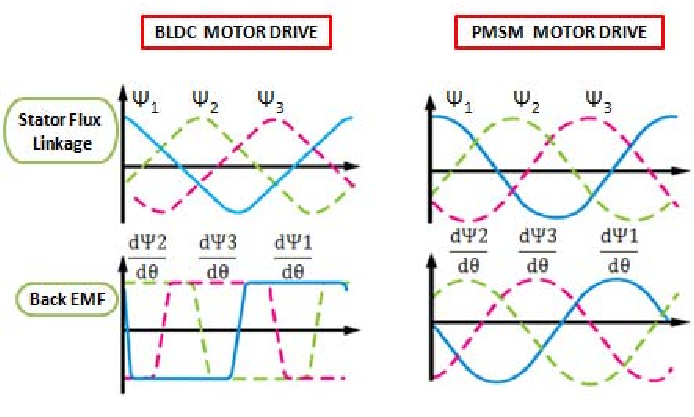
\includegraphics[scale=0.5]{./3_Stand_der_Technik/Abbildungen/PMSM_Back-EMF_1}
			\caption{Back-EMF Synchronmaschine\cite{Rode2023}}
	\end{figure}
	
	\subsubsection{Hall-Sensoren}
		Hall-Sensoren k�nnen sind Halb
	
	\subsubsection{Resolver}